\section{Cubical Type Theory}

Despite providing a strong paradigm shift, HoTT lacks good computational properites.
In particular, Univalence being an axiom breaks computational canonicity, and normalization is not known to hold.~\cite{HoTT}
This is troublesome for computational theorem proving applications, motivating a computationally well-behaved alternative. 

HoTT affords a standard presheaf model in simplicial sets.~\cite{kapulkin2021simplicial}  
Simplices offer poor constructive behaviour.~\cite{bezem2015non} Alternatively, models in cubical sets instead, which being described by products instead of joins, are 
combinatorially nicer. We shall describe cubical sets and their computationally preferable behaviour in type theory. 

\subsection{Cubical Sets}
Let there be a fixed disrete and countable set of \emph{names} $\A$ and define the set of \emph{endpoints} $\2 = \{0,1\}$.
\begin{definition}[The cubical category $\cube$~\cite{bezem2014model}]
  The cubical category $\cube$ has as objects finite subsets $I, J, K... \subseteq \A$.
  A morphism $f : I \to J$ is a set function $f : I \to J \cup \2$, such that 
  $f x = f y$ implies $x = y$ for $x,y \notin \2$. 
  The composition of morphisms $f : I \to J$ and $g : J \to K$ is defined as 
    $g \circ f (x) = g(f(x))$ when $f x \notin \2$ and $f x$ otherwise.
  
\end{definition}
We will call morphisms \emph{substitutions} as they encode substituting names to ${0,1}$. 
We will also denote $fg$ for $g \circ f$ as well as $xf$ for $f(x)$ from now on (called diagram order),
and often omit braces from finte sets of names like $I \cup \{x, y\}$ or $I - \{x,y\}$. 

For $I \subseteq J$, we call the inclusion $f : I \to J$ a \emph{degeneracy map}. 
We have the \emph{face maps} $(x = 0), (x = 1) : I  \to I - x$ sending $x$ to $0$ and $1$ respectively. (Note how these constructions parallel the simplex category ${\Delta})$

\begin{definition}[Cubical sets]
  A cubical set $X$ is a covariant functor $X : \cube \to \Set$, i.e., a presheaf over $\cube^{op}$.
\end{definition}
That is, a cubical set $X$ is a collection of sets $X(I)$ and for any substitution $f : I \to J$, set functions $X(I) \to X(J)$, $u \mapsto uf$ such that $u\1 = u$ and $u(fg) = (uf)g$.
This can be thought of as $X(\varnothing)$ is the set of points of a space, $X(x)$ are its lines, $X(x,y)$ are squares, and so on.
{
\setlength{\abovedisplayskip}{0pt}
 \setlength{\belowdisplayskip}{0pt}
\[
\begin{tikzpicture}[>=stealth, scale=0.9]

% Corner nodes
  \node (A) at (0,0) {$u_{00}$};
  \node (B) at (3,0) {$u_{10}$};
  \node (C) at (0,2) {$u_{01}$};
  \node (D) at (3,2) {$u_{00}$};

% Center label
\node at (1.5,1) {$u$};

% Edges with labels
\draw[->] (A) -- node[below] {$u(y = 0)$} (B);
\draw[->] (C) -- node[above] {$u(y = 1)$} (D);
\draw[->] (A) -- node[left] {$u(x = 0)$} (C);
\draw[->] (B) -- node[right] {$u(x = 1)$} (D);
% extend bounding box to the right
\path (C.north west); % ensure top-left is included
\path (D.south east) ++(2,0); % extend right side

% define a point safely to the right, centered vertically
\coordinate (E) at ($(C)!0.5!(A) + (5,0)$);

% draw axes
\draw[->] (E) -- ++(0.8,0) node[right] {$x$};
\draw[->] (E) -- ++(0,0.8) node[above] {$y$};
\end{tikzpicture}
\]
}

Cubical sets form a presheaf category, i.e. $\cSet := [\square, \Set]$ with morphisms given by 
natural transformations.
\begin{example}[Interval] 
  The interval $\I$ is the cubical set defined by $\I(I) = I \cup \2$ and for $f : I \to J$,
  $\I(f)$ is the extension of the set theoretic map of $f$ such that $\I(f)(0) = 0$
  and $\I(f)(1) = 1$.
\end{example}

Note that for a fixed name $x$, $\I \cong \mathbf{y}\{x\}$, where $\mathbf{y}$ is the Yoneda embedding.
More generally, $\cube_I = \mathbf{y}I$ where $I$ contains $n$ elements, is the representable $n$-cube.

\begin{definition}[Non-dependent Path Space]  
  Given a cubical set $X$, we define its \emph{path space} $[\I]X$ as a cubical set $([\I]X)(I) = X(I,x_I)$ where $x_I$ is a fresh name $x_I \notin I$.
  Let $f : I \to J$ be a sustitution, then $X(f)$ is given by the induced map from $f$ via inclusion, composed with substituting $x_I$ for $x_J$, i.e.,
  $\omega (X(f))= \omega f(x_I = x_J)$.
\end{definition}
For a cubical set $X$, $[\I]X$ is also a cubical set. $[\I]X(\varnothing)$ are the lines in $X$, $[\I]X(x)$ are the squares in $X$, $[\I]X(x,y)$ are the cubes in $X$,
and so on.

\begin{definition}[Non-dependent Identity Type]
  Given a cubical set $X$, and $a, b \in X(\varnothing)$, the \emph{identity type} $\Id_X(a,b)$ is the subobject of $[\I]X$ such that
  $\omega \in (\Id_X(a,b))(I)$ iff there is some name $x \in I$ such that $\omega(x =  0) = a$ and $\omega(x = 1) = b$. 
\end{definition}

\subsection{The Uniform Kan Condition}

\begin{definition}[Open boxes] 
  Let $X$ be a cubical set. Let $I$ be a finite set of names, and $x, J \subseteq I$, with $x \notin J$, the direction in which the box will be open.
  Fix $a$ either $0$ or $1$.
  An \emph{open box} denoted $\vec{u}$ is a family of faces $u_{yb}$ in $X(I - y)$ for each $(y,b)$ either $(x,a)$ or $y \in J, b = 0,1$,
  such that \[u_{yb} (z = a) = u_{za}(y = b)\] for all $y, z \in J, y \neq z$ and $b = 0, 1$.
\end{definition}
The idea is that an open box contains all faces, except for one face in a direction $x$, and $a$ corresponds to the face present in $x$.

\begin{definition}[Kan Cubical Set]
  A Kan cubical set $X$ is a cubical set $X$, equipped with \emph{filling operations} $X\fillup$, and $X\filldown$,
  such that for every $J,x \subseteq I, x \notin J$, there are $X\fillup \vec{u}, X \filldown \vec{u}$ in $X(I)$, where $\vec{u}$ is an open box
  with $u_{x0}$ and $u_{x1}$ in $X(I - x)$ in the respective cases $X \fillup \vec{u}$ and $X \filldown \vec{u}$, such that the following condition holds:
  \[
    (X \fillup \vec{u})(y = b) = u_{yb} \text{ \emph{and} } (X \filldown \vec{u})(y = b) = u_{yb}
  \]
  along with the {`uniformity'} or {`coherence'} condition, that for $f : I \to K$ defined on $J,x$, we require:
  \[
    (X \fillup \vec{u}) f = X \fillup (\vec{u} f) \text{\emph{ and }} (X \filldown \vec{u}) f = X \filldown (\vec{u} f) \]
\end{definition}
We also denote $X^{+} \vec{u} = X \fillup \vec{u} (x = 1)$ and $X^{-} \vec{u} = X \filldown \vec{u} (x = 0)$.
This condition for $X$, known as the \emph{Kan condition} is the analogous statement to \emph{``every horn has a filler"} from Kan complexes, that is, \emph{``every open box has a filler"}.
\[
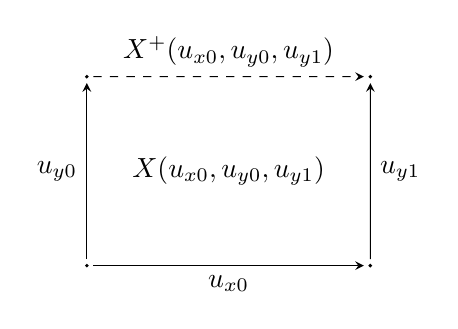
\begin{tikzpicture}[scale=1.2, >=stealth]
  \node[circle, fill, inner sep=0.5pt] (A) at (0,0) {};
  \node[circle, fill, inner sep=0.5pt] (B) at (3,0) {};
  \node[circle, fill, inner sep=0.5pt] (C) at (0,2) {};
  \node[circle, fill, inner sep=0.5pt] (D) at (3,2) {};


  % Corner nodes (filled dots)
  \node[circle, inner sep=1.5pt] (A) at (0,0) {};
  \node[circle, inner sep=1.5pt] (B) at (3,0) {};
  \node[circle, inner sep=1.5pt] (C) at (0,2) {};
  \node[circle, inner sep=1.5pt] (D) at (3,2) {};

  % Edges (arrows automatically stop at node boundary)
  \draw[->] (A) -- node[below] {$u_{x0}$} (B);
  \draw[->] (A) -- node[left] {$u_{y0}$} (C);
  \draw[->] (B) -- node[right] {$u_{y1}$} (D);

  % Dashed top edge
  \draw[->, dashed] (C) -- node[above] {$X^{+} (u_{x0},u_{y0},u_{y1})$} (D);

  % Interior label
  \node at (1.5,1) {$X \fillup (u_{x0},u_{y0},u_{y1})$};

\end{tikzpicture}
\]

\subsection{Conclusion}

Any presheaf category gives rise to a model of dependent type theory by intepreting each presheaf as a type.~\cite{hofmann97} 
Hence, cubical sets form such a model with (dependent) products, (dependent) sums, inductive types and identity types.
We refine this model by restricting to Kan Cubical Sets taken along with a specified `Kan Structure',
which are the Kan filling operations $X \fillup$ and $X \filldown$. This is needed in order to justify the elimination rules for identity types.~\cite{bezem2014model}

Due to computation of paths via cubes simply being a matter of substitution, since paths in $A$ are functions $\I \to A$, we obtain a
computational realization of equality.
Consequently, we can prove functional extentionality, univalence, and canonicity for HITs.~\cite{bezem2019univalence, huber2019canonicity}
For a complete, formal treatment of cubical sets and their semantics, see ~\cite{huberphd, cohen2016cubical}.
